
\documentclass[letterpaper,10pt]{article}
\usepackage[top=0.75in, bottom=0.75in, left=0.75in, right=0.75in]{geometry}
\usepackage[english]{babel}
\usepackage{amsmath}
\usepackage{amssymb,amsfonts,textcomp}
\usepackage{color}
\usepackage{array}
\usepackage{supertabular}
\usepackage{hhline}
\usepackage{hyperref}
\usepackage{float}
\usepackage{type1cm}
\hypersetup{pdftex, colorlinks=true, linkcolor=blue, citecolor=blue, filecolor=blue, urlcolor=blue, pdftitle=SYSTEMS AND SOFTWARE REQUIREMENTS SPECIFICATION (SSRS) TEMPLATE, pdfauthor=Clinton Jeffery, pdfsubject=, pdfkeywords=}
\usepackage[pdftex]{graphicx}
% Outline numbering
\setcounter{secnumdepth}{5}
\renewcommand\thesection{\arabic{section}}
\renewcommand\thesubsection{\arabic{section}.\arabic{subsection}}
\renewcommand\thesubsubsection{\arabic{section}.\arabic{subsection}.\arabic{subsubsection}}
\renewcommand\theparagraph{\arabic{section}.\arabic{subsection}.\arabic{subsubsection}.\arabic{paragraph}}
\renewcommand\thesubparagraph{\arabic{section}.\arabic{subsection}.\arabic{subsubsection}.\arabic{paragraph}.\arabic{subparagraph}}
\makeatletter
\newcommand\arraybslash{\let\\\@arraycr}
\makeatother
% Page layout (geometry)
\usepackage{geometry}
\geometry{textheight=8.5in, textwidth=6in}
% Footnote rule
\setlength{\skip\footins}{0.0469in}
\renewcommand\footnoterule{\vspace*{-0.0071in}\setlength\leftskip{0pt}\setlength\rightskip{0pt plus 1fil}\noindent\textcolor{black}{\rule{0.25\columnwidth}{0.0071in}}\vspace*{0.0398in}}
% Pages styles
\makeatletter
\newcommand\ps@Standard{
  \renewcommand\@oddhead{\selectlanguage{english}\rmfamily\color{black} Oregon State University CapStone Team 41 \hfill}
  \renewcommand\@evenhead{\@oddhead}

  \renewcommand\@evenfoot{\@oddfoot}
  \renewcommand\thepage{\arabic{page}}
}
\newcommand\ps@Convertviii{
  \renewcommand\@oddhead{}
  \renewcommand\@evenhead{\@oddhead}
  \renewcommand\@oddfoot{}
  \renewcommand\@evenfoot{\@oddfoot}
  \renewcommand\thepage{\arabic{page}}
}
\newcommand\ps@Convertvii{
  \renewcommand\@oddhead{}
  \renewcommand\@evenhead{\@oddhead}
  \renewcommand\@oddfoot{}
  \renewcommand\@evenfoot{\@oddfoot}
  \renewcommand\thepage{\arabic{page}}
}
\newcommand\ps@Convertvi{
  \renewcommand\@oddhead{}
  \renewcommand\@evenhead{\@oddhead}
  \renewcommand\@oddfoot{}
  \renewcommand\@evenfoot{\@oddfoot}
  \renewcommand\thepage{\arabic{page}}
}
\newcommand\ps@Convertv{
  \renewcommand\@oddhead{}
  \renewcommand\@evenhead{\@oddhead}
  \renewcommand\@oddfoot{}
  \renewcommand\@evenfoot{\@oddfoot}
  \renewcommand\thepage{\arabic{page}}
}
\newcommand\ps@Convertiv{
  \renewcommand\@oddhead{}
  \renewcommand\@evenhead{\@oddhead}
  \renewcommand\@oddfoot{}
  \renewcommand\@evenfoot{\@oddfoot}
  \renewcommand\thepage{\arabic{page}}
}
\newcommand\ps@Convertii{
  \renewcommand\@oddhead{}
  \renewcommand\@evenhead{\@oddhead}
  \renewcommand\@oddfoot{}
  \renewcommand\@evenfoot{\@oddfoot}
  \renewcommand\thepage{\arabic{page}}
}
\newcommand\ps@FirstPage{
  \renewcommand\@oddhead{}
  \renewcommand\@evenhead{\@oddhead}
  \renewcommand\@oddfoot{}
  \renewcommand\@evenfoot{\@oddfoot}
  \renewcommand\thepage{\arabic{page}}
}
\makeatother
\pagestyle{Standard}
\setlength\tabcolsep{1mm}
\renewcommand\arraystretch{1.3}
% footnotes configuration
\makeatletter
\renewcommand\thefootnote{\arabic{footnote}}
\makeatother
\title {The Client Requirements Document of App and website for Health Sciences Careers in Oregon }
\author{Zixuan Feng
	   Jason Ye
	   David Corbelli }
\date{October, 2016}
\begin{document}
\clearpage\setcounter{page}{1}\pagestyle{Standard}
\thispagestyle{FirstPage}

\bigskip

{\centering\selectlanguage{english}\bfseries\color{black}
The Client Requirements Document of App and website for Health Sciences Careers in Oregon
\par}


\bigskip

{\centering\selectlanguage{english}\bfseries\color{black}
Version 1.0, 2016-10-26
\par}


 \vspace{2cm}
\noindent 
Zixuan Feng \\
Email: fengzi@oregonstate.edu\\
Address: 1148 Kelley Engineering Center, 2500 NW Monroe Ave, Corvallis, OR 97331\\
Tel:5419086066\\

 \vspace{1cm}
\noindent 
Jason Ye \\
Email:yeja@oregonstate.edu\\
Address: 1148 Kelley Engineering Center, 2500 NW Monroe Ave, Corvallis, OR 97331\\
Tel:5033800809\\

 \vspace{1cm}
\noindent 
David Corbelli \\
Email:Corbelld@oregonstate.edu\\
Address: 1148 Kelley Engineering Center, 2500 NW Monroe Ave, Corvallis, OR 97331\\
Tel:5038863960\\










\bigskip

\clearpage{\centering\selectlanguage{english}\bfseries\color{black}
The Client Requirements Document FOR


\bigskip

{\centering\selectlanguage{english}\bfseries\color{black}
App and website for Health Sciences Careers in Oregon
\par}


\bigskip


\bigskip



\begin{figure}
\centering

\end{figure}

\bigskip


\bigskip

{\centering\selectlanguage{english}\bfseries\color{black}
Version 1.0
\par}

{\centering\selectlanguage{english}\bfseries\color{black}
2016-10-26
\par}


\bigskip


\bigskip

{\centering\selectlanguage{english}\bfseries\color{black}
Prepared for:
\par}

{\centering\selectlanguage{english}\bfseries\color{black}
Oregon Department of Education
\par}


\bigskip


\bigskip

{\centering\selectlanguage{english}\bfseries\color{black}
Prepared by:
\par}

{\centering\selectlanguage{english}\bfseries\color{black}
Team: Cap 41
\par}

{\centering\selectlanguage{english}\bfseries\color{black}
Oregon State University
\par}



\clearpage{\centering\selectlanguage{english}\bfseries\color{black}
[App and website for Health Sciences Careers in Oregon] SSRS
\par}


\bigskip

{\centering\selectlanguage{english}\bfseries\color{black}
RECORD OF CHANGES
\par}


\bigskip

\begin{flushleft}
\tablehead{}
\begin{supertabular}{|m{0.47685984in}|m{0.6087598in}|m{1.3587599in}|m{0.23375985in}|m{2.0462599in}|m{0.7337598in}|m{0.6330598in}|}
\hline
~

\centering \selectlanguage{english}\color{black} Version &
~

\centering \selectlanguage{english}\color{black} Date of finished &
~

\centering \selectlanguage{english}\color{black} Location of change
(e.g., page or figure \#) &
\centering \selectlanguage{english}\bfseries\color{black} A\newline
M\newline
D &
~

~

\centering \selectlanguage{english}\color{black} description
change &
~

\centering \selectlanguage{english}\color{black} Approved/ No Approved (initials)
&
~

\centering\arraybslash \selectlanguage{english}\color{black} Date
Approved\\\hline
~
 &
~
 &
~
 &
~
 &
~
 &
~
 &
~
\\\hline
~
 &
~
 &
~
 &
~
 &
~
 &
~
 &
~
\\\hline
~
 &
~
 &
~
 &
~
 &
~
 &
~
 &
~
\\\hline
~
 &
~
 &
~
 &
~
 &
~
 &
~
 &
~
\\\hline
~
 &
~
 &
~
 &
~
 &
~
 &
~
 &
~
\\\hline
~
 &
~
 &
~
 &
~
 &
~
 &
~
 &
~
\\\hline
~
 &
~
 &
~
 &
~
 &
~
 &
~
 &
~
\\\hline
~
 &
~
 &
~
 &
~
 &
~
 &
~
 &
~
\\\hline
~
 &
~
 &
~
 &
~
 &
~
 &
~
 &
~
\\\hline
~
 &
~
 &
~
 &
~
 &
~
 &
~
 &
~
\\\hline
~
 &
~
 &
~
 &
~
 &
~
 &
~
 &
~
\\\hline
~
 &
~
 &
~
 &
~
 &
~
 &
~
 &
~
\\\hline
~
 &
~
 &
~
 &
~
 &
~
 &
~
 &
~
\\\hline
~
 &
~
 &
~
 &
~
 &
~
 &
~
 &
~
\\\hline
~
 &
~
 &
~
 &
~
 &
~
 &
~
 &
~
\\\hline
~
 &
~
 &
~
 &
~
 &
~
 &
~
 &
~
\\\hline
~
 &
~
 &
~
 &
~
 &
~
 &
~
 &
~
\\\hline
~
 &
~
 &
~
 &
~
 &
~
 &
~
 &
~
\\\hline
~
 &
~
 &
~
 &
~
 &
~
 &
~
 &
~
\\\hline
~
 &
~
 &
~
 &
~
 &
~
 &
~
 &
~
\\\hline
~
 &
~
 &
~
 &
~
 &
~
 &
~
 &
~
\\\hline
~
 &
~
 &
~
 &
~
 &
~
 &
~
 &
~
\\\hline
~
 &
~
 &
~
 &
~
 &
~
 &
~
 &
~
\\\hline
~
 &
~
 &
~
 &
~
 &
~
 &
~
 &
~
\\\hline
\end{supertabular}
\end{flushleft}





{\selectlanguage{english}\color{black}
\foreignlanguage{english}{*}\foreignlanguage{english}{\textbf{A}}\foreignlanguage{english}{
- ADDED
\ }\foreignlanguage{english}{\textbf{M}}\foreignlanguage{english}{ -
MODIFIED
\ }\foreignlanguage{english}{\textbf{D}}\foreignlanguage{english}{ -
DELETED}}

\clearpage{\centering\selectlanguage{english}\bfseries\color{black}
\foreignlanguage{english}{\MakeUppercase{\ }}\foreignlanguage{english}{\MakeUppercase{App and website for Health Sciences Careers in Oregon}}
\par}

%%%%%%%%%%%%%%%%%%%%%%%%%%%%%%%%Head page%%%%%%%%%%%%%%%%%%%%%%%%%%%%%%%%%%%%%%%%
{\centering\selectlanguage{english}\bfseries\color{black}
CONTENTS
\par}


\bigskip

{\selectlanguage{english}\bfseries\color{black}
Section\ \ 1}

\setcounter{tocdepth}{9}
\renewcommand\contentsname{}
\tableofcontents

\bigskip

\clearpage\clearpage\setcounter{page}{1}\pagestyle{Convertii}
\section[Abstract]{\selectlanguage{english}\rmfamily\bfseries\color{black}
Abstract}
{\selectlanguage{english}\color{black}\normalsize(10pt)\emph{
The application and website for Oregon health science careers is a guide for middle school and high school level students to learn about careers within the field of health sciences . Between an application and website, the service shall provide information as exploration tool for students looking for future careers in health science. Due to the many fields under the classification of health and science, it may be difficult for a student beginning to take an interest in the subject to find the proper path they are looking for. As a development team we will focus on developing an exploratory website and then develop corresponding applications for two major platforms, Android and iOS. Through our platform, students will explore pathways and careers in health and science. In this paper, we will discuss our design and specifications of the applications and website we plan to develop.}}


\subsection[Definition]{\selectlanguage{english}\rmfamily\bfseries\color{black}
Definition}
{\selectlanguage{english}\itshape\color{black}\normalsize(default)
At the middle school and high school level, students begin taking an interest in their future career paths. For many, it remains unclear how to take first steps towards their future careers and what requirements they will need to fulfill. Within the field of health and sciences, there exist many branching paths to explore before making an informed definitive choice can be made; the major umbrellas of health sciences include therapeutic services, diagnostics, health informatics, support services, as well as research and development. Each each of these departments separate and divide further into more specific fields. It is important that students are able to distinguish between the different fields in order to make an educated choice and without an organized platform it may be difficult for students to identify which option is most suited for them.}


\subsection[Solution]{\selectlanguage{english}\rmfamily\bfseries\color{black}
Solution}
{\selectlanguage{english}\itshape\color{black}\normalsize(10pt)
In order to bridge this gap in information, we shall build a website with the purpose of education and career path exploration that will allow students, along with their parents, teachers, and counselors, to develop an understanding of what each career option encompasses. This area of the site will detail information specifying the differences between classifications of health services and what duties can be expected of an individual in such a position. Informative pages pertaining to career paths will branch into increasingly specific fields in order for students to pinpoint their options. Along with career exploration, we will also open up navigation and development for pages such as information on health education centers, workforce partners, educators, and current events news. For convenience, we will also develop a mobile app counterpart with information linked to the website that allows the capability to bookmark specific pages for later viewing. With this platform, students will have the information required to pursue a career in health sciences.}

\subsection[Performance Metrics]{\selectlanguage{english}\rmfamily\bfseries\color{black}
Performance Metrics}
{\selectlanguage{english}\itshape\color{black}\normalsize(10pt)
In order to measure our work, we need to know what is working and what is not for both the website and our applications. Towards this end, we will provide a website and application prototype for user-based testing. The prototype would allow us to examine and analyze our objective: whether or not we can assist students in finding a field in health sciences that interests them. We would be collecting and testing feedback to see which information is useful and which is not for our audience. In addition, we shall perform script testing, where a user is given a set of tasks to complete in order, which it will help us discover problems in the projects design. It is important for us to know whether or not the user can find or access a certain feature on the website and application given certain scenarios. These tests tend to produce benefits for usability metrics and generate qualitative data. Our goal is to provide a user-friendly way for students to explore different career paths, thus ensuring a quality user-interface is necessity. Once we have completed development and our user-tests return all positive experiences we may conclude that we have reached our goal..}

%%%%%%%%%%%%%%%%%%%%%%%%%%%%%%%%Section one%%%%%%%%%%%%%%%%%%%%%%%%%%%%%%%%%%%%%%%

\bigskip


\clearpage\section[Requirements Document]{\selectlanguage{english}\rmfamily\bfseries\color{black}
Requirements Document}


\subsection[PRODUCT
PERSPECTIVE]{\selectlanguage{english}\rmfamily\bfseries\color{black}
PRODUCT PERSPECTIVE}
{\selectlanguage{english}\itshape\color{black}\normalsize(10pt)
{The goal for this project is to provide a website and application for Oregon health science careers. This project allows students, parents, teachers, and counselors to explore current pathways and health science careers. The website displays pages containing information pertaining to the separate branches of health science careers; each page may also provide links to pages with more specific fields. There is also navigation supported for pages including educator tools, workforce partners, and education centers. The majority of the website information will be stored in a database for easy manipulation. Additionally a mobile companion application will be available based upon a mobile web browser to provide an alternative viewing platform.}



\subsection[PRODUCT
FUNCTIONS]{\selectlanguage{english}\rmfamily\bfseries\color{black}
PRODUCT FUNCTIONS}
{\selectlanguage{english}\itshape\color{black}\normalsize(10pt)
The website designed for Health and Science Careers in Oregon allows users to interact through both web browsers and mobile devices. Users are able to navigate through a series of informative pages to learn about the different fields within health sciences. Alternatively, users may also use a search bar to view pages that include desired keywords. The website is also designed for mobile viewing and includes the same features as the desktop site.}


\subsection[USER
CHARACTERISTICS]{\selectlanguage{english}\rmfamily\bfseries\color{black}
USER CHARACTERISTICS}
{\selectlanguage{english}\itshape\color{black}\normalsize(default)
The website is focused for middle and high school level students. Students at this level begin to choose their future career paths and to some it is still unclear how to start their goals and what requirements they need to fulfill. This website is meant to bridge this gap and provide an opportunity for exploration and learning. }

\subsection[CONSTRAINTS]{\selectlanguage{english}\rmfamily\bfseries\color{black}
CONSTRAINTS}
{\selectlanguage{english}\itshape\color{black}\normalsize(10pt)
The application for mobile devices may be constrained by differences in mobile devices based on display size. There exist many different display sizes and aspect ratios to take into account. Network connection is also a constraining factor as information is pulled not only from a web server, but also from a database. Should connection be poor, the required time for a page to load may vary, along with the time it takes to query the database.}


\subsection[ASSUMPTIONS AND
DEPENDENCIES]{\selectlanguage{english}\rmfamily\bfseries\color{black}
ASSUMPTIONS AND DEPENDENCIES}
{\selectlanguage{english}\itshape\color{black}\normalsize(10pt)
Detailed information concerning careers in health sciences is provided by an affiliate of the Oregon Department of Education. Additionally, a secure hosting server and database for the final product will also be provided by the Oregon Department of Education. Publishing of the mobile application will also be handled by the Oregon Department of Education.}



\subsection[Additional Requirements]{\selectlanguage{english}\rmfamily\bfseries\color{black}
Additional Requirements}
{\selectlanguage{english}\itshape\color{black}\normalsize(10pt)
The timeframe of this project will be estimated by this Gantt chart, while our progress will be tracked separately.} 

\begin{figure}[H]
\subsubsection[Timeframe:]{\selectlanguage{english}\rmfamily\bfseries\color{black}
Timeframe:}
\centering
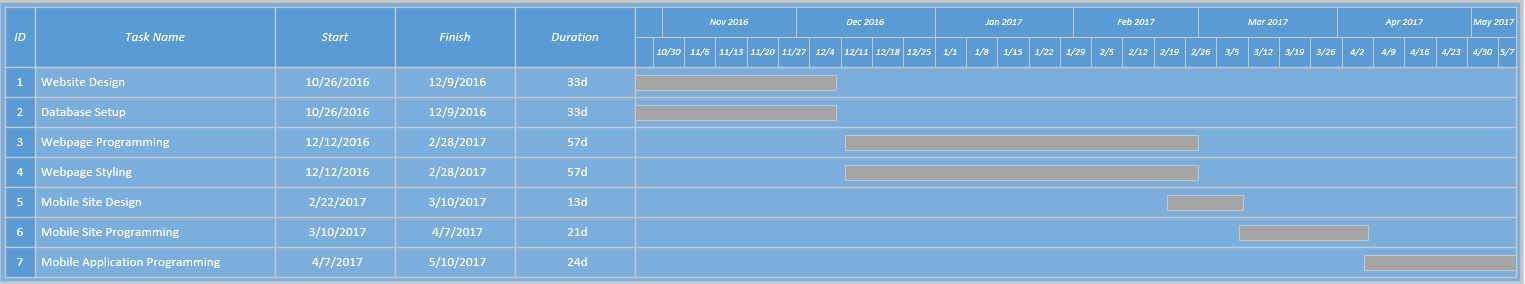
\includegraphics[width=15cm,height=4cm]{Gantt.JPG}
\end{figure}
\end{document}